\documentclass{article}
\usepackage{nips15submit_e}

\newcommand{\fix}{\marginpar{FIX}}
\newcommand{\new}{\marginpar{NEW}}
\usepackage{amssymb}
\usepackage{bm}
\usepackage{latexsym}
\usepackage{amsmath}
\usepackage{url}
\usepackage{graphicx}
\usepackage{hyperref}
\usepackage{hyperref}
\hypersetup{
    bookmarks=true,         
    unicode=true,  
    colorlinks=true,       
    linkcolor=blue,          
    citecolor=blue,       
    filecolor=blue,      
    urlcolor=blue          
}
\usepackage[ruled,vlined]{algorithm2e}
\usepackage{pstricks,pst-plot,pst-text,pst-tree,pst-eps,pst-fill,pst-node,pst-math}
\usepackage{caption}
\usepackage{subcaption}

\title{Latent Dirichlet allocation}
\author{
J\'er\^ome DOCK\`ES (\texttt{jerome\{at\}dockes.org}) \\
\textbf{Pascal LU (\texttt{pascal.lu\{at\}student.ecp.fr})} \\
\'Ecole Normale Sup\'erieure de Cachan \\
}

\begin{document}

\maketitle

\section{Latent Dirichlet allocation}
\subsection{Presentation of the model}

We consider the problem of modeling text corpora. The goal is to find short descriptions of the members of a collection that enable efficient processing of large collections while preserving the essential statistical relationships that are useful for basic tasks such as classification, novelty detection, summarization, and similarity and relevance judgments.

\medskip

\textbf{Notations}
\begin{itemize}
\setlength\itemsep{-0.2em}
  \item $\mathcal{D} = \{d_{1},d_{2}, \ldots, d_{M}\}$ is a corpus (collection of $M=|\mathcal{D}|$ documents). We denote $|\mathcal{D}|$ (\verb"num_docs") the number of documents.
  \item $\mathcal{V}$ is the vocabulary. Its size is denoted $V$ (\verb"voc_size").
  \item The number of topics is denoted $k$ (\verb"num_topics").
\end{itemize}

For a document $d \in \mathcal{D}$,
\begin{itemize}  
\setlength\itemsep{-0.2em}
%  \item $d = (w_1, \ldots, w_{n(d)})$ represents the document $d$ of the corpus $^{(d)}$, composed of a sequence of $n(d)$ words.
  \item $d = (w_1^{(d)}, \ldots, w_{N_d}^{(d)})$ represents the document $d$, where the $w_i^{(d)}$ are all distinct. $N_d$ (\verb"doc_size") is the number of \textbf{distinct}\footnote{For implementation issues, this representation for a document is smaller than the representation proposed by \cite{BNJ03}.} words in the document $d$.
  \item $w^{(d)}$ (\verb"word_incidences") is an matrix containing the number of times each word in the vocabulary appears in the document. The size of $w^{(d)}$ is the number of distinct words in document $d$ $\times$ vocabulary size ($N_d \times V$).
 %   $w_{nj}^{(d)} = \begin{cases} 1 & \text{if the word in position } n \text{ of the document is the word in position } j \text{ of the dictionary} \\ 0 & \text{otherwise} \end{cases}$
 \item $\theta^{(d)}$ is an array of size $k$, representing a probability density.
 \item $z^{(d)}$ is the set of topics : $z_{ni}^{(d)} =  1$ if the word $n$ is linked with the topic $i$. Hence, it is a matrix of size $N_d \times k$.
\end{itemize}

\medskip

Latent Dirichlet allocation (LDA) is a generative probabilistic model of a corpus. The main idea is that documents are represented as random mixtures over latent topics, where each topic is characterized by a distribution over words. 

\begin{algorithm}
\caption{Generative process}
\KwData{corpus $\mathcal{D}$}
\Begin{
\For{\emph{each document} $d \in \mathcal{D}$}{
Choose $N \sim \textnormal{Poisson}(\xi)$\;
Choose $\theta^{(d)} \sim \textnormal{Dir}(\alpha)$\;
\For{\emph{each of the $N$ words $w_n^{(d)}$}}{
Choose a topic $z_n^{(d)} \sim  \textnormal{Multinomial}(\theta^{(d)})$\;
Choose a word $w_n$ from $p(w_n |z_n^{(d)}, \beta)$, a multinomial probability conditioned on the topic $z_n^{(d)}$.
}
}
}
\end{algorithm}

\begin{figure}[ht!]
\begin{center}
\psset{xunit=1.0cm,yunit=1.0cm,algebraic=true,dimen=middle,dotstyle=o,dotsize=5pt 0,linewidth=0.8pt,arrowsize=3pt 2,arrowinset=0.25}
\begin{pspicture*}(-0.5,-0.3)(8,3.5)
\rput(0,1){\pscirclebox[linecolor=black,fillstyle=solid,fillcolor=blue]{\textcolor{white}{$\alpha_j$}}}
\rput(2,1){\pscirclebox{$\theta^{(d)}_j$}}
\rput(4,1){\pscirclebox{$z^{(d)}_{nj}$}}
\rput(6,1){\pscirclebox[linecolor=black,fillstyle=solid,fillcolor=yellow]{$w_{nj}^{(d)}$}}
\rput(6,3){\pscirclebox[linecolor=black,fillstyle=solid,fillcolor=blue]{\textcolor{white}{$\beta_{jv}$}}}
\pspolygon(3.25,0.25)(7.2,0.25)(7.2,1.75)(3.25,1.75)
\pspolygon(1.25,0)(7.75,0)(7.75,2)(1.25,2)
\psline{->}(0.27,1)(1.58,1)
\psline{->}(2.43,1)(3.58,1)
\psline{->}(4.44,1)(5.5,1)
\psline{->}(6,2.7)(6,1.5)
\rput(6.75,0.5){$N_d$}
\rput(7.5,0.25){$M$}
\end{pspicture*}
\caption{Generative model}
\label{generative}
\end{center}
\end{figure}

The following parameters are introduced:
\begin{itemize}
  \item $\alpha$ (\verb"dirich_param") is an estimate of the parameter of the dirichlet distribution which generates the parameter for the (multinomial) probability distribution over topics in the document. The size of $\alpha$ is the number of topics, $k$. \textbf{We suppose that $\alpha = \alpha \mathbf{1}_{k}$\footnote{This assumption is suggested by the authors of \cite{BNJ03}.} .}
  
  \item $\beta$ (\verb"word_prob_given_topic") is a matrix of size (number of topics $\times$ vocabulary size $= k \times V$) which gives the (estimated) probability that a given topic will generate a certain word:
\[ \beta_{ij}= p(w^j = 1 | z^i = 1) \]
 \end{itemize}

LDA is based on the computation of the parameters $(\alpha, \beta)$, for instance by maximizing the log-likelihood. For a document $d$, the probability $p(d|\alpha, \beta)$ is given by:

\begin{align*}
p(d|\alpha, \beta) 
& = \int p(\theta^{(d)}|\alpha) \left( \prod_{n=1}^{N_{d}} p(w_n^{(d)}|\theta^{(d)}, \beta)\right) \text{d}\theta  \\
& = \int p(\theta^{(d)}|\alpha) \left( \prod_{n=1}^{N_{d}} \sum_{z_n^{(d)}} p(z_n|\theta^{(d)}) p(w_n^{(d)}|z_n^{(d)}, \beta)\right) \text{d}\theta  \\
& = \frac{\Gamma\left( \sum_i \alpha_i\right)}{\prod_i \Gamma(\alpha_i)} \int \left( \prod_{i=1}^k (\theta_i^{(d)})^{\alpha_i - 1} \right) \left( \prod_{n=1}^{N_d} \sum_{i=1}^k \prod_{j=1}^V (\theta_i^{(d)} \beta_{ij})^{w_{nj}^{(d)}} \right) \text{d}\theta
\end{align*}

\subsection{Inference and parameter estimation}

The basic idea of variational inference is to use Jensen's inequality to obtain an adjustable lower bound on the log likelihood.

For each document $d \in \mathcal{D}$, the following latent variables are introduced:
 \begin{itemize}
\setlength\itemsep{-0.2em}
  \item $\gamma^{(d)}$ (\verb"var_dirich") the variational parameter for the dirichlet distribution. The size of $\gamma^{(d)}$ is the number of topics, $k$.
  \item $\phi^{(d)}$ (\verb"var_multinom") the variational parameter for the multinomial distribution The size of $\phi^{(d)}$ is (number of distinct words in document $d$ $\times$ number of topics), $N_d \times k$.
  
  $\phi_{ni}^{(d)}$ depends on the relation between the word in position $n$ of the document and the topic $i$ of the list of topics.
   \end{itemize}

and to try to estimate them instead of $\theta^{(d)}$ and $z_n^{(d)}$. The conditional probability is:

\[ q(\theta^{(d)}, z^{(d)}|\gamma^{(d)}, \delta^{(d)}) = q(\theta^{(d)}|\gamma^{(d)}) \prod_{n=1}^{N_d} q(z_n^{(d)}|\phi_n^{(d)})\]

\begin{figure}[ht!]
\begin{center}
\begin{subfigure}{.75\textwidth}
\begin{center}
\psset{xunit=1.0cm,yunit=1.0cm,algebraic=true,dimen=middle,dotstyle=o,dotsize=5pt 0,linewidth=0.8pt,arrowsize=3pt 2,arrowinset=0.25}
\begin{pspicture*}(-0.5,-0.3)(8,3.5)
\rput(0,1){\pscirclebox[linecolor=black,fillstyle=solid,fillcolor=blue]{\textcolor{white}{$\alpha_j$}}}
\rput(2,1){\pscirclebox{$\theta^{(d)}_j$}}
\rput(4,1){\pscirclebox{$z^{(d)}_{nj}$}}
\rput(6,1){\pscirclebox[linecolor=black,fillstyle=solid,fillcolor=yellow]{$w_{nj}^{(d)}$}}
\rput(6,3){\pscirclebox[linecolor=black,fillstyle=solid,fillcolor=blue]{\textcolor{white}{$\beta_{jv}$}}}
\pspolygon(3.25,0.25)(7.2,0.25)(7.2,1.75)(3.25,1.75)
\pspolygon(1.25,0)(7.75,0)(7.75,2)(1.25,2)
\psline{->}(0.27,1)(1.58,1)
\psline{->}(2.43,1)(3.58,1)
\psline{->}(4.44,1)(5.5,1)
\psline{->}(6,2.7)(6,1.5)
\rput(6.75,0.5){$N_d$}
\rput(7.5,0.25){$M$}
\end{pspicture*}
\caption{Generative model}
\label{generative}
\end{center}
\end{subfigure}
\begin{subfigure}{.75\textwidth}
\begin{center}
\psset{xunit=1.0cm,yunit=1.0cm,algebraic=true,dimen=middle,dotstyle=o,dotsize=5pt 0,linewidth=0.8pt,arrowsize=3pt 2,arrowinset=0.25}
\begin{pspicture*}(-1,-0.1)(4,5)
\rput(0,3){\pscirclebox[linecolor=black,fillstyle=solid,fillcolor=green]{$\gamma^{(d)}_j$}}
\rput(0,1){\pscirclebox{$\theta^{(d)}_j$}}
\rput(2,3){\pscirclebox[linecolor=black,fillstyle=solid,fillcolor=green]{$\phi^{(d)}_{nj}$}}
\rput(2,1){\pscirclebox{$z^{(d)}_{nj}$}}
\pspolygon(1.25,0.25)(3.15,0.25)(3.15,3.75)(1.25,3.75)
\pspolygon(-0.9,0)(3.8,0)(3.8,4)(-0.9,4)
\psline{->}(0,2.5)(0,1.5)
\psline{->}(2,2.5)(2,1.5)
\rput(2.75,0.5){$N_d$}
\rput(3.5,0.25){$M$}
\end{pspicture*}
\caption{Variational model}
\label{variational}
\end{center}
\end{subfigure}
\caption{Graphical model}
\end{center}
\end{figure}

\subsubsection*{EM algorithm}

\begin{algorithm}
\caption{EM algorithm}
\KwData{Corpus $\mathcal{D}$ of documents, number of topics $k$}
\KwResult{\texttt{dirich$\_$param} ($\alpha$), \texttt{word$\_$prob$\_$given$\_$topic} ($\beta$)}
\Begin{
\For{\emph{each} $d \in \mathcal{D}$}{
Compute \texttt{word$\_$incidences} ($w^{(d)}$).
}

Initialize \texttt{dirich$\_$param} ($\alpha$) with a uniform vector of size $k$\;
Initialize \texttt{word$\_$prob$\_$given$\_$topic} ($\beta$) \;

\bigskip

\While{\emph{the expected log-likelihood has not converged}}{
\For{\emph{each} $d \in \mathcal{D}$}{
\texttt{var$\_$dirich} ($\gamma^{(d)}$), \texttt{var$\_$multinom} ($\phi^{(d)}$) = apply \textbf{E-step} to each document $d$ given \texttt{word$\_$incidences} ($w^{(d)}$), \texttt{dirich$\_$param} ($\alpha$), \texttt{word$\_$prob$\_$given$\_$topic} ($\beta$)
}

\texttt{dirich$\_$param} ($\alpha$), \texttt{word$\_$prob$\_$given$\_$topic} ($\beta$) = Apply \textbf{M-step} given $\{$\texttt{word$\_$incidences} ($w^{(d)}$), \texttt{var$\_$dirich} ($\gamma^{(d)}$), \texttt{var$\_$multinom} ($\phi^{(d)}$), $d \in \mathcal{D}\}$.
}
}
\end{algorithm}

The expected log-likelihood for a document $d$, is:
\begin{align*}
L(\gamma^{(d)}, \phi^{(d)}, \alpha, \beta)
& = \log \Gamma\left( k\alpha \right) - k \log \Gamma(\alpha) + (\alpha - 1)  \sum_{i=1}^k \left( \Psi(\gamma_i^{(d)}) - \Psi\left( \sum_{j=1}^k \gamma_j^{(d)} \right) \right) \\
&+ \sum_{n=1}^{N_d} \sum_{i=1}^k \phi_{ni}^{(d)} \left( \Psi(\gamma_i^{(d)}) - \Psi\left( \sum_{j=1}^k \gamma_j^{(d)} \right) \right) \\
&+ \sum_{n=1}^{N_d} \sum_{i=1}^k \sum_{j=1}^V \phi_{ni}^{(d)} w_{nj}^{(d)} \log \beta_{ij} \\
& - \log \Gamma \left( \sum_{j=1}^k \gamma_j^{(d)} \right) + \sum_{i=1}^k \log \Gamma(\gamma_i^{(d)}) - \sum_{i=1}^k(\gamma_i^{(d)} - 1) \left( \Psi(\gamma_i^{(d)}) - \Psi\left( \sum_{j=1}^k \gamma_j^{(d)} \right)\right) \\
&- \sum_{n=1}^{N_d} \sum_{i=1}^k \phi_{ni}^{(d)}\log\phi_{ni}^{(d)} 
\end{align*}

\begin{algorithm}
\caption{E-step for a document $d$ (Variational Inference Procedure)}
\KwData{\texttt{word$\_$incidences} ($w^{(d)}$), \texttt{dirich$\_$param} ($\alpha$), \texttt{word$\_$prob$\_$given$\_$topic} ($\beta$)}
\KwResult{\texttt{var$\_$dirich} ($\gamma^{(d)}$), \texttt{var$\_$multinom} ($\phi^{(d)}$)}
\Begin{
Initialize $\phi_{ni}^{(d)} = \frac{1}{k}$ for all $i$ and $n$\;
Initialize $\gamma_i^{(d)} = \alpha + \frac{1}{k}\sum_{n=1}^{N_d} w_n^{(d)}$ for all $i$ \;
\While{\emph{the expected log-likelihood for the document $d$ has not converged}}{
\For{$n=1\ldots N_d$}{
\For{$i=1\ldots k$}{
$\phi_{ni}^{(d)} = \beta_{iw_n^{(d)}}\exp(\Psi(\gamma_i^{(d)}))$
}
normalize $\phi_n^{(d)}$ to sum to $1$.
}
$\gamma^{(d)} = \alpha + \sum_{n=1}^{N_d} w_n^{(d)} \phi_n^{(d)}$
}
}
\end{algorithm}

\begin{algorithm}
\caption{M-step}
\KwData{$\{$\texttt{word$\_$incidences} ($w^{(d)}$), \texttt{var$\_$dirich} ($\gamma^{(d)}$), \texttt{var$\_$multinom} ($\phi^{(d)}$), $d \in \mathcal{D}\}$}
\KwResult{\texttt{dirich$\_$param} ($\alpha$), \texttt{word$\_$prob$\_$given$\_$topic} ($\beta$)}
\Begin{
$\beta \propto \sum_{d \in \mathcal{D}} (\phi^{(d)})^{\top}w^{(d)}$ (which corresponds to $\beta_{ij} \propto \sum_{d \in \mathcal{D}} \sum_{n=1}^{N_d} \phi_{ni}^{(d)} w_{nj}^{(d)}$)

\While{\emph{$\alpha$ has not converged}}{
$\alpha \leftarrow \alpha - \frac{L'(\alpha)}{L''(\alpha)}$ where \[ \begin{cases}L'(\alpha) = |\mathcal{D}| k \left[ \Psi\left( k \alpha \right) - \Psi(\alpha)\right] + \sum_{d \in \mathcal{D}} \left[ \sum_{i=1}^k \Psi (\gamma_i^{(d)}) - \Psi\left( \sum_{j=1}^k \gamma_j^{(d)}\right) \right] \\
L''(\alpha) = |\mathcal{D}|k [k\Psi'(k \alpha) - \Psi' \left( \alpha\right)] \end{cases} \]
}
}
\end{algorithm}

\section{Implementation and results}
\subsection{Implementation issues}

The following algorithm was implemented :

\begin{algorithm}
\caption{EM algorithm implemented}
\KwData{Corpus $\mathcal{D}$ of documents, number of topics $k$}
\KwResult{\texttt{dirich$\_$param} ($\alpha$), \texttt{word$\_$prob$\_$given$\_$topic} ($\beta$)}
\Begin{
\For{\emph{each} $d \in \mathcal{D}$}{
Compute \texttt{word$\_$incidences} ($w^{(d)}$).
}

Initialize \texttt{dirich$\_$param} ($\alpha$)\;
Initialize \texttt{word$\_$prob$\_$given$\_$topic} ($\beta$) \;
Initialize \texttt{sum$\_$psi$\_$var$\_$dirich} ($\Sigma_{\gamma}$) = 0 \;
\bigskip

\While{\emph{the expected log-likelihood $L(\mathcal{D}, \alpha, \beta)$ has not converged}}{
Initialize expected log-likelihood $L(\mathcal{D}, \alpha, \beta) = 0$ \;
\For{\emph{each} $d \in \mathcal{D}$}{
\texttt{var$\_$dirich} ($\gamma^{(d)}$), \texttt{var$\_$multinom} ($\phi^{(d)}$) = apply \textbf{E-step} to each document $d$ given \texttt{word$\_$incidences} ($w^{(d)}$), \texttt{dirich$\_$param} ($\alpha$), \texttt{word$\_$prob$\_$given$\_$topic} ($\beta$)

Update $\beta \leftarrow \beta +  (\phi^{(d)})^{\top}w^{(d)}$ \;
Update $\Sigma_{\gamma} \leftarrow \Sigma_{\gamma} + \sum_{i=1}^k \Psi (\gamma_i^{(d)}) - \Psi\left( \sum_{j=1}^k \gamma_j^{(d)}\right) $ \;
Update $L(\mathcal{D}, \alpha, \beta) \leftarrow L(\mathcal{D}, \alpha, \beta) + L(\gamma^{(d)}, \phi^{(d)}, \alpha, \beta)$\;
}

Normalize $\beta$ \;

\While{\emph{$\alpha$ has not converged}}{
$\alpha \leftarrow \alpha - \frac{L'(\alpha)}{L''(\alpha)}$ where $\begin{cases}L'(\alpha) = |\mathcal{D}| k \left[ \Psi\left( k \alpha \right) - \Psi(\alpha)\right] + \Sigma_{\gamma} \\
L''(\alpha) = |\mathcal{D}|k [k\Psi'(k \alpha) - \Psi' \left( \alpha\right)] \end{cases}$
}
}
}
\end{algorithm}

\textbf{Computation of $\gamma^{(d)}$}: With the original formula, we have: $\sum \gamma^{(d)} = N_d\times \alpha + \textnormal{number of words in the document } d$.

%Another formula for $\gamma^{(d)}$:
%\[ \gamma^{(d)} \leftarrow \gamma^{(d)} + \left( \sum_{n=1}^{N_d} w_n^{(d)} \phi_n^{(d), \text{old}} - w_n^{(d)} \phi_n^{(d), \text{new}} \right) \]

\textbf{Log-likelihood}: $\Gamma(x)$ becomes exponentially big when $x \rightarrow \infty$. We will prefer working with $\ln \Gamma(x)$ (\texttt{gammaln} in scipy) instead of $\Gamma(x)$ (or \texttt{numpy.log(gamma)}).

\textbf{Initialization}:
\begin{itemize}
  \item $\alpha$ is chosen randomly, but $\alpha \neq 0$.
  \item $\beta$ is chosen randomly.
\end{itemize}

\subsection{Results}

The database we used may be found at the address \url{http://www.daviddlewis.com/resources/testcollections/reuters21578/}.

\begin{table}[ht!]
\begin{center}
\begin{tabular}{c c c c}
\hline
\textbf{Topic 1} & \textbf{Topic 2} & \textbf{Topic 3}  & \textbf{Topic 4}\\
\hline
devices & prolonged & zestril & features \\
disk & council & annesthetic &  shipping  \\
megabyte & forum & hypertension & 798  \\
expandable & dissident & oth & 998  \\
megabytes & flying & statil & sells  \\
equipped &  sparks & diabetic & AppleWorld  \\
monochrome &talks & complications & Conference  \\
peripheral & outweighed & Barbara & 899  \\
color & accomplishments & definitive & science  \\
\hline
\end{tabular}
\caption{Results for 4 topics $(k=10)$}
\end{center}
\end{table}

\subsubsection*{Convergence of the expected log-likelihood on the corpus}

The following curve represents the evolution of the expected log-likelihood computed on the whole corpus:

\begin{figure}[ht!]
\begin{center}
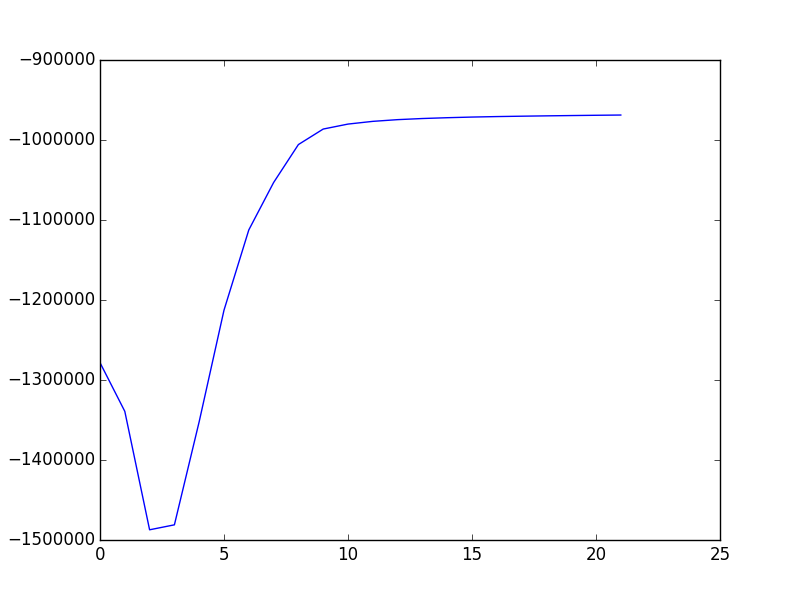
\includegraphics[width=0.5\linewidth]{img/figure_1.png}
\caption{Expected log-likelihood for a corpus ($k=30$)}
\end{center}
\end{figure}

\subsubsection*{Convergence of the expected log-likelihood for a document (variational inference)}




\section{Conclusion}

\begin{thebibliography}{BNJ03}
\bibitem[BNJ03]{BNJ03} David M. Blei, Andrew Y. Ng and Michael I. Jordan. Latent Dirichlet Allocation. \emph{The Journal of Machine Learning Research}, 3:993--1022, 2003.
\end{thebibliography}


\end{document}